\paragraph{Lavpass} \mbox{} \\
Husk at reaktansen $X_C$ er avhengig av frekvens.
$$X_C = \frac{1}{2\pi f C}$$
Det tilsier at reaktansmotstanden blir lavere med høy frekvens.
\\\\
La oss se hva dette gjør med spenningen
over kondensatoren i en RC-krets.
\\
\begin{circuitikz} \draw
(0,0) to[vsourcesin, label=$Vs$] (0,2)
      to[R, label=$R$] (4,2)
      to[C, label=$X_C$] (4,0)
      -- (0,0)
(4,2) to[short, -o] (5,2)
(4,0) to[short, -o] (5,0)
      ;
\end{circuitikz}
\\
Spenningsdeling (husk: 90 grader forskyvning) for $X_C$ gir oss
$$V_{ut} = \frac{X_C}{\sqrt{X_C^2 + R^2}} \cdot V_S$$
Dette viser at spenningen ut blir lavere ved høy frekvens.
\\
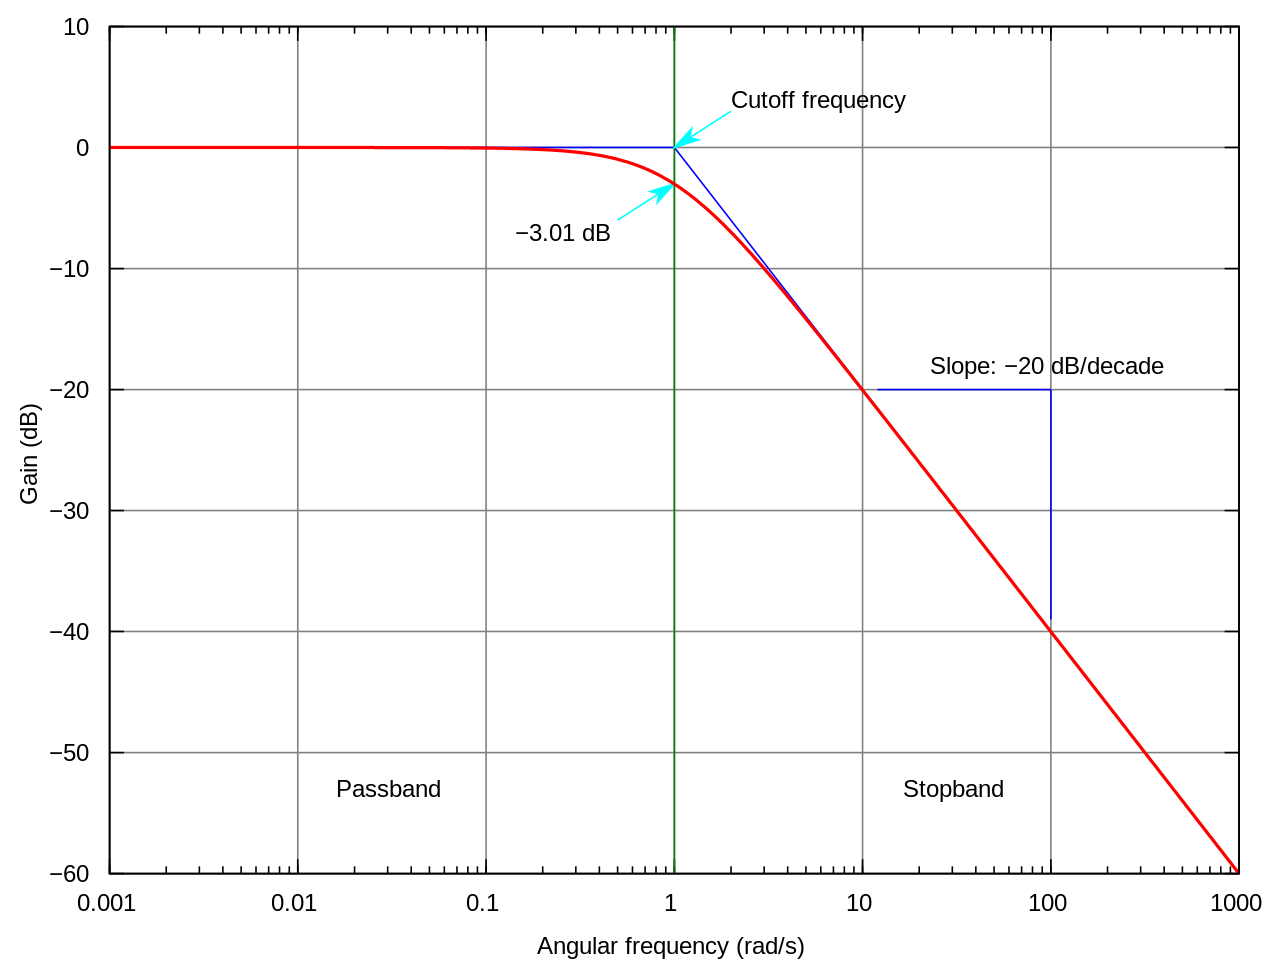
\includegraphics[width=\textwidth]{./img/lowpass}
\\
Cutoff (grense) frekvensen får man når $X_C = R$.
$$f_g = \frac{1}{2\pi R C}$$



\paragraph{Høypass} \mbox{} \\
TODO



\paragraph{Eksempel} \mbox{} \\
TODO
